\chapter{Mandelbrot percolation - methods and results}
\label{ch:mandelbrot_experimental}

\section{Introduction}

Now we turn our attention to the so called Mandelbrot percolation, which is also known in the literature as Fractal percolation. The idea is, again, to study the clusters structure and distribution, but the coloring of the lattice happens in a different way: instead of doing a single pass over the lattice and coloring the nodes at random, we do this process repeatedly - at each step, we subdivide each node in the lattice into a number of "sub-nodes" and color the remaining "alive" (not yet colored) nodes with probability $p$. An illustration of this process can be seen in \autoref{fig:mandelbrot_process}. 
Each iteration generates a lattice $A_n$ (which is, of course, highly correlated with the previous lattice $A_{n-1}$). Mandelbrot percolation is the study of the limit of this process the number of steps increases arbitrarily, that, is $\lim_{n\to\infty} A_n$.

\section{Simulation methods}

The simulations were run, again, on a 2D periodic square lattice. 
We studied three properties: the percolation probability, mean cluster size and percolating cluster strength. We explicitly used exactly the same definitions, methods and algorithms as for the 2D case - the reason for this is that this way, a direct comparison is possible. The precise description of these methods is available in \autoref{ch:classical_experimental}.




\begin{figure}[H]
  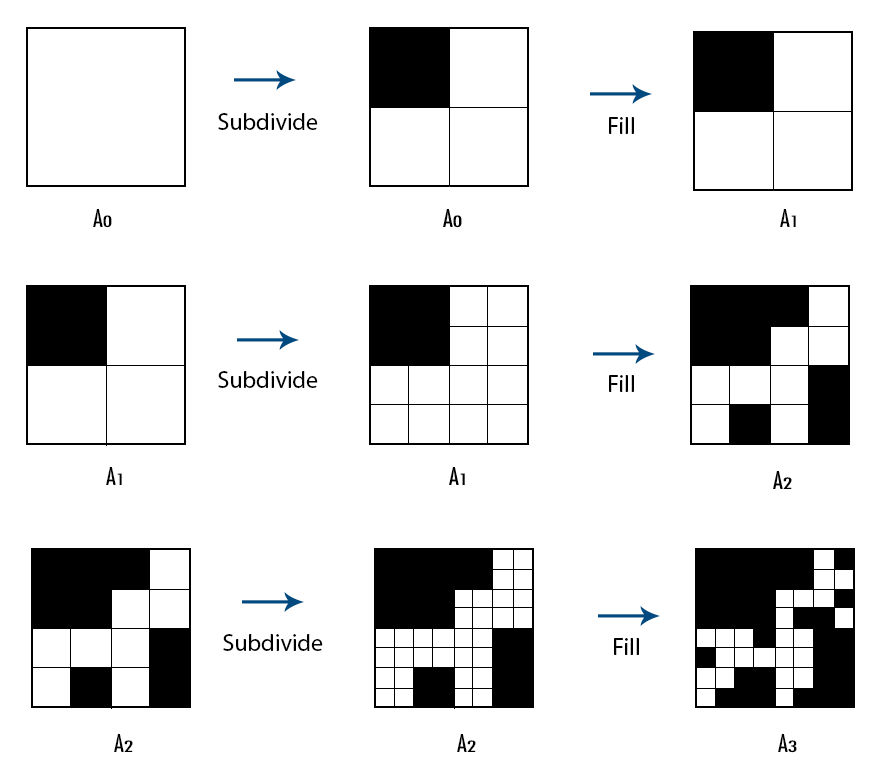
\includegraphics[width=\linewidth]{Images/mandelbrot_process.png}
  \caption{Illustration of the Mandelbrot percolation iteration process, showing three iterations}
  \label{fig:mandelbrot_process}
\end{figure}



\begin{figure}[H]
  \includegraphics[width=\linewidth]{Images/mandelbrot_lattice.png}
  \caption{A Mandelbrot percolation lattice after 11 iterations}
  \label{fig:mandelbrot_lattice}
\end{figure}



\section{Percolation probability}


\begin{figure}[H]
  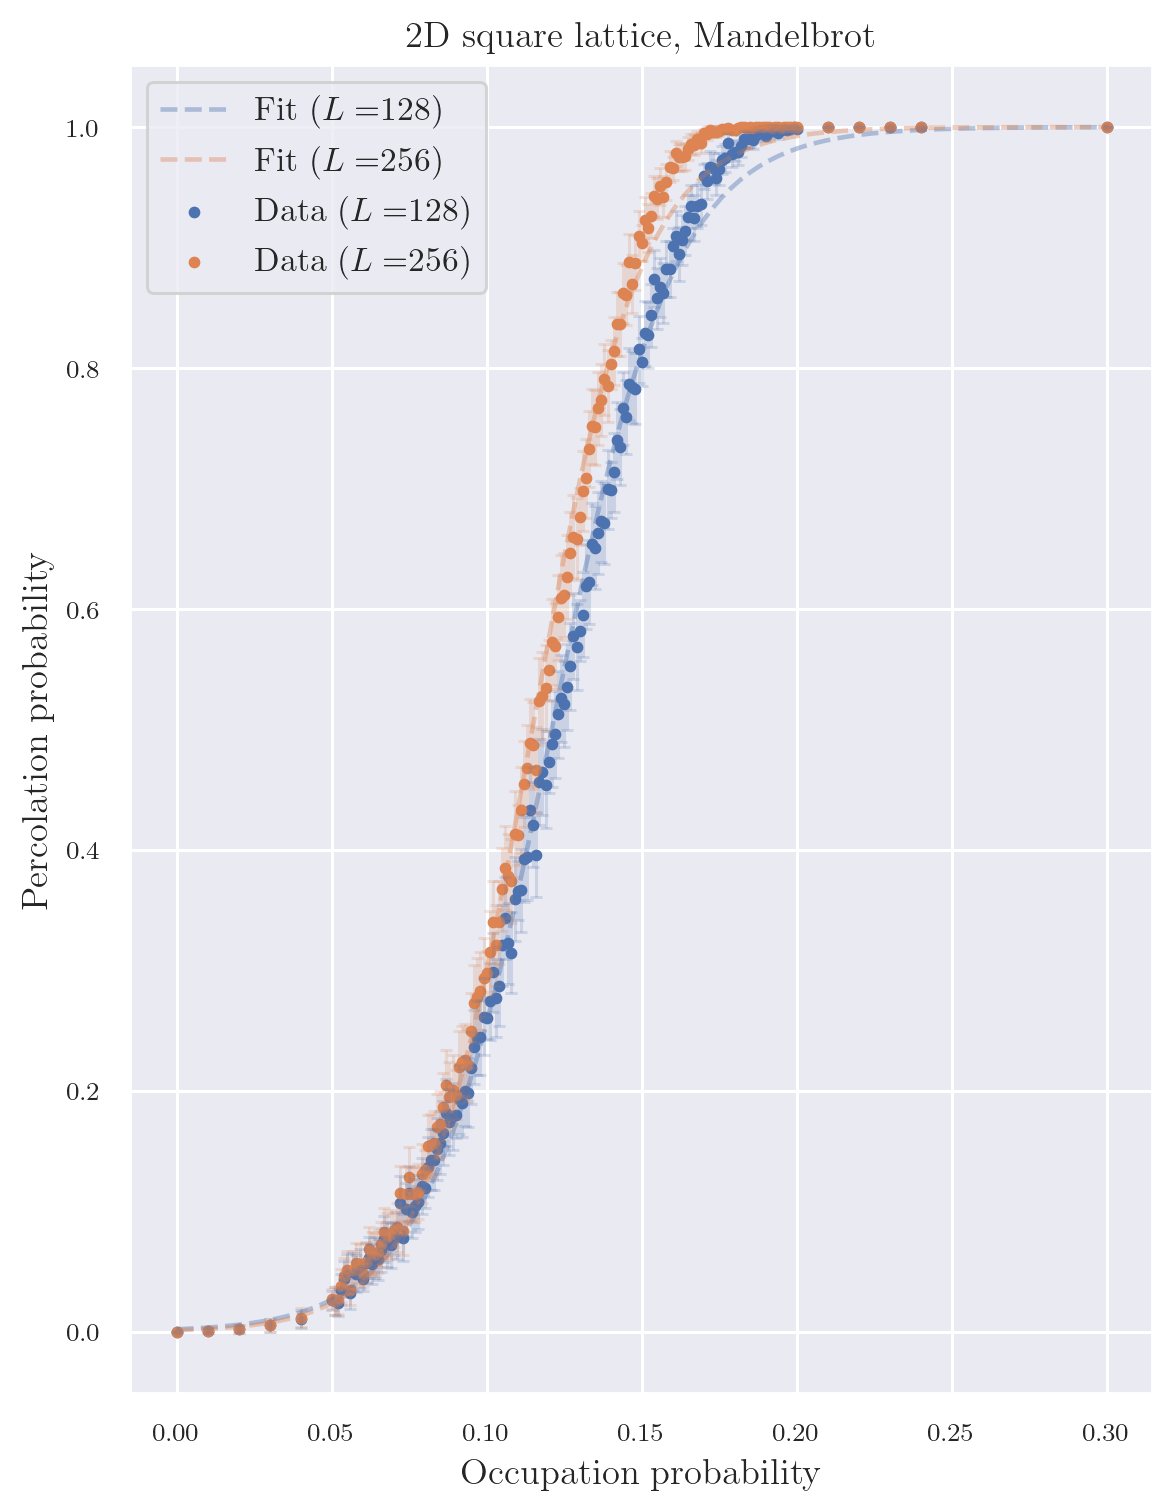
\includegraphics[width=\linewidth]{Images/simm_perc_prob_2.png}
  \caption{Percolation probability for the Mandelbrot percolation model}
  \label{fig:simm_perc_prob_2}
\end{figure}

\section{Percolating cluster strength}


\begin{figure}[H]
  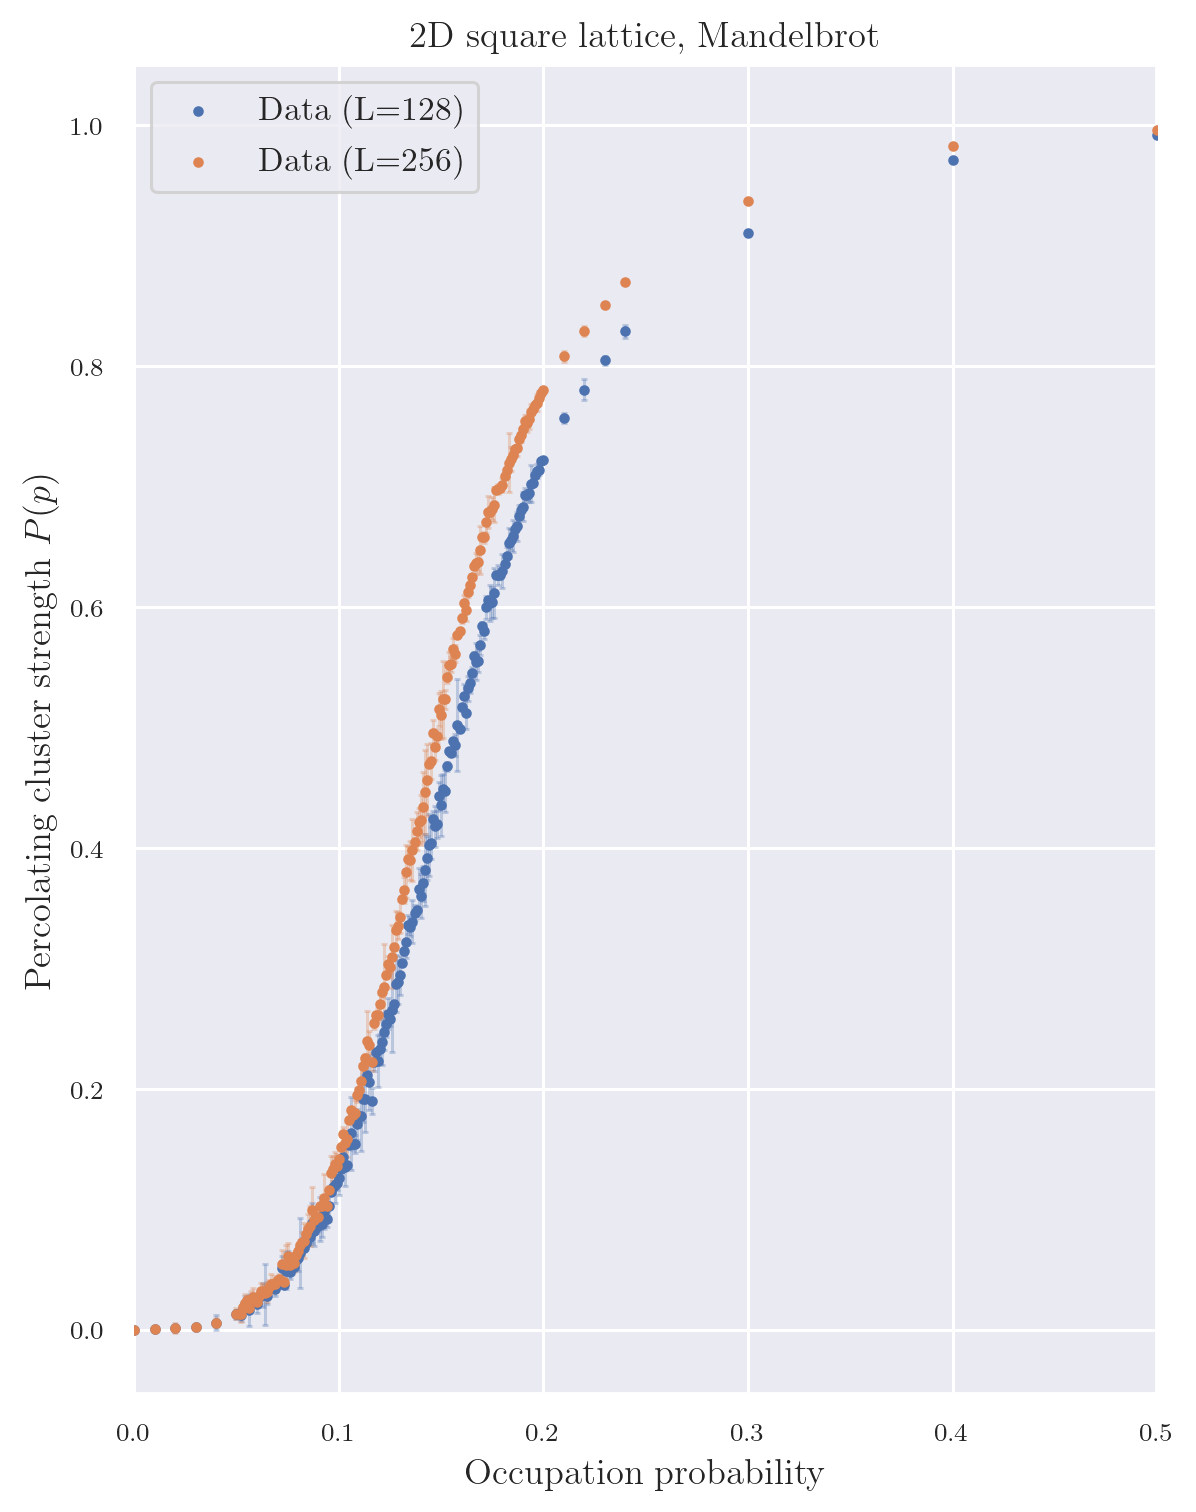
\includegraphics[width=\linewidth]{Images/simm_perc_clust_strength_1.png}
  \caption{Percolation probability for the Mandelbrot percolation model}
  \label{fig:simm_perc_clust_strength_1}
\end{figure}


\section{Mean cluster size}


\begin{figure}[H]
  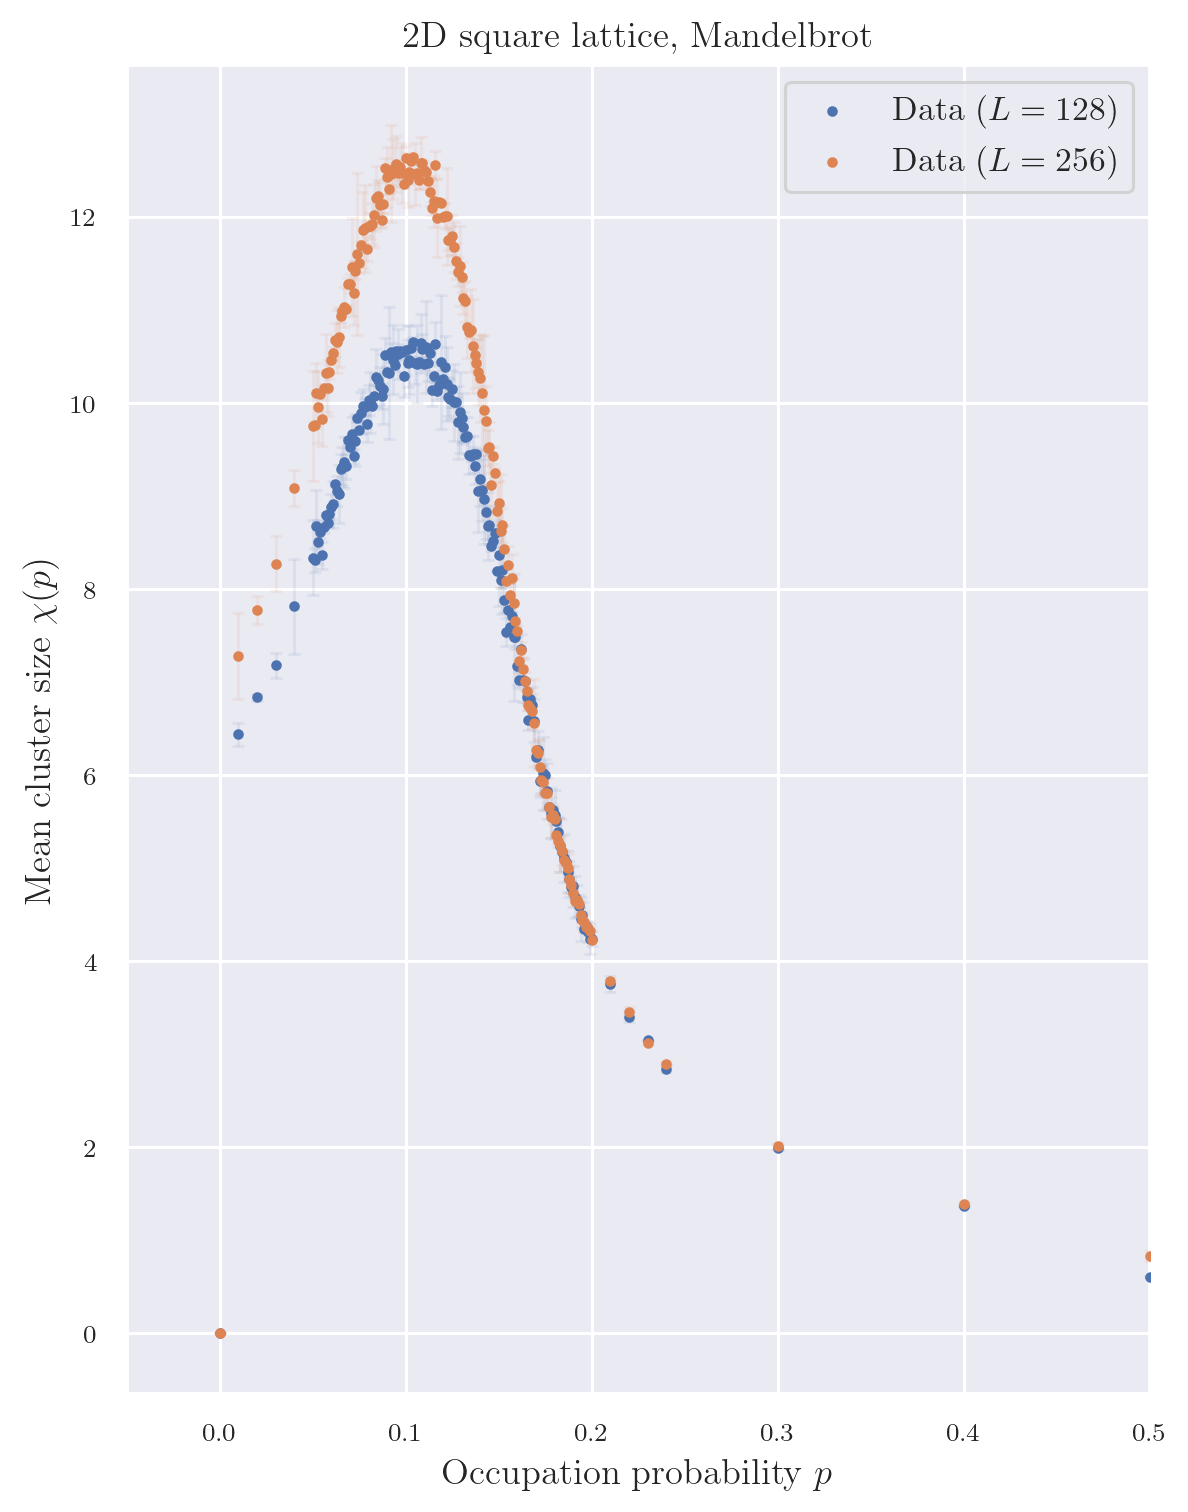
\includegraphics[width=\linewidth]{Images/simm_mean_cluster_size_1.png}
  \caption{Percolation probability for the Mandelbrot percolation model}
  \label{fig:simm_mean_cluster_size_1}
\end{figure}


